\chapter{\label{chap:simulation}Sistemas e Simulações}

De acordo com Banks~(2005, p.~3):

\begin{directcite}
Simulação é a imitação da operação de um sistema ou processo do mundo real ao
longo do tempo. Ela envolve a geração de uma história artificial de um sistema
ou processo e a observação desta história de modo a realizar inferências a
respeito das características operacionais da realidade ali representada.
\end{directcite}

Entretanto, a simulação não é a única abordagem existente para se estudar e
compreender um sistema e suas características. É senso comum que cada sistema,
possuindo suas próprias características e idiossincrasias, deve ser analisado
através da ferramenta correta. Logo, embora a simulação pareça ser uma boa
alternativa à primeira vista em diversos casos, é possível que ela não seja a
forma mais apropriada para o seu estudo. Assim, se faz importante a existência
de métodos objetivos para que se possa verificar se a simulação é realmente a
ferramenta apropriada para cada caso estudado.

\section{\label{chap:waystostudy}Formas de Estudar um Sistema}

Ao realizar o estudo sobre um sistema e seu comportamento, uma gama de
estratégias podem ser colocadas em prática, dentre as quais podemos citar:

\begin{itemize}
\item Experimentar com o próprio sistema;
\item Experimentar com um modelo físico do sistema;
\item Experimentar com um modelo matemático do sistema.
\end{itemize}

A fim de decidir de forma objetiva qual a melhor abordagem para um dado sistema,
Law~\cite{Law} propõe uma reflexão (figura~\ref{fig:systemstudy}) através das
seguintes perguntas:

\begin{figure}[htb!]
\centering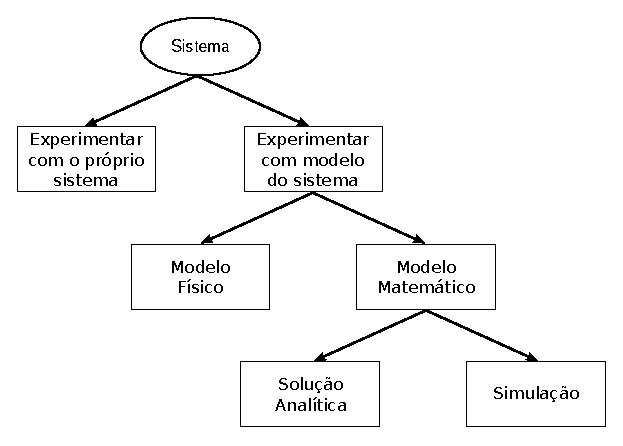
\includegraphics{img/systemstudy.eps}
\caption{\label{fig:systemstudy}Formas de estudar um sistema. Fonte:~\cite{Law}}
\end{figure}

\begin{enumerate}
\item \textit{Experimentar com o próprio sistema ou experimentar com um modelo do mesmo?}

Caso exista viabilidade técnica e financeira na alteração de um sistema e na
observação de sua operação sob estas novas condições, é desejável que se faça as
experimentações diretamente no próprio sistema. Entretanto, frequentemente esta
alternativa é inviável por diversas razões, dentre as quais encontram-se:

\begin{itemize}
  \item O custo dos experimentos é muito elevado:

  \textbf{Exemplo}: construir uma instalação para um novo elevador em um prédio
já existente.

  \item O impacto causado pelos experimentos pode ser prejudicial ao sistema:

  \textbf{Exemplo}: um mercado deseja reduzir o número de atendentes em caixas a
fim de diminuir seus custos operacionais e aumentar seus lucros. Porém, esta
medida pode causar um aumento significativo no tamanho das filas - e,
consequentemente, um aumento no tempo de espera dos cliente, podendo até causar
desistências.

  \item O sistema não existe:

  \textbf{Exemplo}: o sistema ainda está nas fases de concepção, projeto ou
desenvolvimento.

\end{itemize}

Por isto, muitas vezes é necessário realizar os experimentos utilizando um
\textit{modelo} em substituição ao sistema real. No escopo desde estudo, um
sistema de elevadores operacional e pronto para realizar as experimentações não
encontra-se entre os recursos disponíveis para a elaboração da pesquisa. Ainda,
mesmo que tal estrutura estivesse disponível, os cenários de testes possíveis
seriam limitados pelas restrições físicas do sistema, tornando o estudo das
melhorias mais caro e menos flexível. Logo, optou-se pela utilização de um
\textit{modelo do sistema}.

\item \textit{Experimentar utilizando um modelo físico do sistema ou utilizar um modelo
matemático?}

Cockpits de aviões desacoplados do resto da nave, automóveis construídos em
escala em túneis de vento e miniaturas funcionais de sistemas de elevadores são
alguns exemplos de \textit{modelos físicos} de sistemas. Ocasionalmente, este
tipo de modelo é utilizado para estudar sistemas de engenharia ou
logística~\cite{Law}. Porém, a vasta maioria dos casos exigem \textit{modelos
matemáticos}. Estes modelos são criados baseados em suposições realizadas a
respeito do funcionamento do sistema. Tais suposições, que normalmente possuem a
forma de relações lógicas e quantitativas, são então avaliadas numericamente
enquanto são coletados dados com o intuito de observar de que forma o sistema
real reagiria.

No contexto deste estudo, um modelo físico de um sistema de elevadores poderia
ser constituído por uma maquete de um prédio com mini-elevadores movidos à
motores de passo, que por sua vez seriam controlados por microcontroladores
programáveis conectados à uma rede de sensores. Este projeto por si só,
entretanto, já seria grandioso demais - além de, obviamente, fugir do escopo da
Ciência da Computação e ser mais adequado à um trabalho de conclusão de
Engenharia Elétrica ou Engenharia de Controle e Automação. Além disso, da mesma
forma que em um sistema real de elevadores, os cenários de testes possíveis
seriam limitados pelas restrições físicas do modelo do sistema. Portanto, optou-
se pela utilização de um \textit{modelo matemático do sistema}, reproduzível em
ambiente computacional e parametrizável para diferentes cenários.

\item \textit{O problema pode ser resolvido de forma analítica?}

De posse de um \textit{modelo matemático de um sistema}, o mesmo deve ser
examinado de modo a verificar de qual modo ele pode ser utilizado para dar
solução ao problema que ele representa. Segundo~\cite{Law}, se o modelo for
simples o suficiente, provavelmente é possível trabalhar com suas relações
matemáticas e equações para obter uma solução exata, anaĺitica. \cite{Law} cita
como exemplo o modelo de mecânica básica $d = vt$, onde $d$ é a distância, $v$ é
a velocidade média e $t$ é o tempo de viagem. Se soubermos a distância a ser
viajada e a velocidade, podemos trabalhar com as equações do modelo e encontrar
a equação $t = d/r$ para encontrar, exatamente, o tempo de viagem. Embora esta
solução seja simples, não é incomum a busca por soluções analíticas tornar-se
extraordinariamente complexa, exigindo vastos recursos computacionais.

Portanto, se uma solução analítica para um problema é conhecida e possui
eficiência computacional, é mais apropriado estudar este sistema desta forma do
que através de simulação. Do contrário, o sistema deve ser estudado através de
simulações~-~ou~seja, através do exercício numérico das entradas do modelo
matemático do sistema e da observação da forma com que tais exercícios afetam as
saídas. Conforme afirmado no capítulo \ref{chap:intro} deste estudo, o problema
de atribuir elevadores para atender chamadas feitas pelos passageiros
minimizando alguma métrica encontra-se no conjunto de problemas NP- difícil (ou
NP-hard, ou NP-complexo)~\cite{SeKo99}. Assim, uma solução ótima, computável em
tempo polinomial, ainda não é conhecida para este problema. Este fato vai ao
encontro dos grandes esforços da indústria em procurar soluções para resolver o
problema ao longo das décadas, não poupando esforços e investimentos em busca
desta solução.

\end{enumerate}

Em outra abordagem, Banks~\cite{BanksGibson} define 10 situações onde a simulação
\textbf{não} é indicada. Tais situações são:

\begin{enumerate}
\item \textit{Quando o problema puder ser resolvido utilizando-se de bom senso}

Conforme discutido anteriormente neste capítulo, dada a complexidade do problema
(NP-completo), não parece ser possível encontrar a solução apenas utilizando o
bom senso e operações básicas.

\item \textit{Quando o problema puder ser resolvido de forma analítica}

Sobre o problema em questão, uma solução anaĺítica ainda é desconhecida.

\item \textit{Quando o problema puder ser resolvido através de experimentos
diretamente no sistema}

Como já constatado, não há um sistema de elevadores instalado para realizar as
experimentações entre os recursos disponíveis para este estudo. E, mesmo que
houvesse, haveria uma imposição de limites nos cenários de testes em função das
restrições físicas do sistema. Logo, não é possível realizar os experimentos
diretamente no sistema.

\item \textit{Quando seus custos da simulação excederem os seus ganhos}

Não foi realizado um estudo e avaliação a respeito dos custos deste estudo,
compreendendo o embasamento, modelagem, projeto e implementação do simulador.
Entretanto, acredita-se que os resultados trarão benefícios aos usuários de
elevadores, conforme defendido nos capítulos \ref{chap:intro},
\ref{chap:problem} e \ref{chap:proposal}.

\item \textit{Quando não há recursos financeiros suficientes}

Idem ao item anterior.

\item \textit{Quando não há tempo suficiente}

De acordo com o cronograma exibido na seção \ref{chap:stages}, acredita-se que
será possível implementar um sistema simulador capaz de fornecer dados em tempo
hábil.

\item \textit{Quando não há dados suficientes, nem mesmo estimativas}

Neste estudo serão utilizadas distribuições de probabilidade baseadas em
estimativas obtidas através de observação e senso comum.

\textbf{TO-DO: Onde observaremos?} % TO-DO

\item \textit{Quando não há possibilidade de verificar a validade do modelo}

\textbf{TO-DO: Como verificaremos a validade do modelo?} % TO-DO

\item \textit{Quando as expectativas e o poder da simulação são superestimados}

Neste estudo, o foco das expectativas está nos ganhos que o uso de algoritmos de
Inteligência Artificial poderão trazer para estes sistemas de elevadores. A
simulação é vista apenas como uma forma para avaliar os resultados obtidos.
Portanto, ela não é superestimada e o objeto de estudo não se enquadra nesta
situação.

\item \textit{Quando o comportamento do sistema é muito complexo ou não pode ser
definido (e.~g. seres humanos)}

Um \textbf{EGCS} não é um sistema de alta complexidade, possuindo um conjunto de
comportamentos limitado e um espaço de estados moderado. Portanto, não se
enquadra nesta situação.

\end{enumerate}

Em função destas reflexões acredita-se que a simulação é uma forma apropriada
para estudar um \textbf{EGCS}.

\section{Classificação do Modelo de Simulação}

A partir de um modelo matemático a ser estudado por meio de simulação (doravante
chamado de \textit{modelo de simulação}), o mesmo pode ser classificado em três
dimensões~\cite{Banks,Law}:

\begin{enumerate}
\item \textit{Estático ou Dinâmico}

Um modelo de simulação estático é uma representação de um sistema em um ponto
particular no tempo, ou então um sistema onde o tempo simplesmente é
irrelevante. Por outro lado, um modelo de simulação dinâmico representa um
sistema que evolui e se modifica com o passar do tempo.

No escopo deste trabalho, o modelo de simulação é claramento dinâmico. Deseja-se
verificar o comportamento do sistema ao longo de um intervalo de tempo finito, à
medida que passageiros chegam e elevadores os transportam através dos andares do
prédio.

\item \textit{Determinístico ou Estocástico}

Um modelo de simulação que não possua nenhum componente probabilístico (i.~e,~
aleatoriedade) é chamado de \textit{determinístico}. Em um modelo de simulação
\textit{determinístico} sua saída é ``determinada'' no momento em que a sua
entrada é definida - mesmo que ainda tome tempo computacional para realizar o
cálculo de qual seja o resultado \cite{Law}. Em outras palavras, significa dizer
que a saída fornecida pelo modelo de simulação será sempre a mesma para uma
mesma entrada. Porém a grande maioria dos sistemas do mundo real possuem, no
mínimo, algum grau de aleatoridade na sua entrada. Estes sistemas dão origem a
modelos de simulação \textit{estocásticos}. Estes, diferentemente de modelos
\textit{determinísticos}, fornecem uma saída igualmente aleatória~-~e, por esta
razão, esta saída deve ser considerada como um conjunto de \textit{estimativas}
das características reais do sistema, e não as características propriamente
ditas \cite{Banks}.

Em um \textbf{EGCS} real não é possível prever quantos passageiros utilizarão o
sistema, quando eles chegarão e tampouco para qual andar irão. Portanto, um
modelo de simulação válido neste escopo deve ser \textit{estocástico} de modo a
lidar com a aleatoridade da entrada de passageiros no sistema.

\item \textit{Contínuo ou Discreto}

A figura \ref{fig:disccont} ilustra o comportamento de uma variável de estado em
modelos de simulação \textit{contínuos} e \textit{discretos}. O modelo
\textit{contínuo} é aquele onde os valores das variáveis mudam continuamente ao
longo do tempo. Já em um modelo \textit{discreto} as variáveis de estado tem seu
valor alterado em instantes separados do tempo \cite{Banks}. É importante
salientar que modelos discretos não necessariamente representam sistemas
discretos e vice-versa \cite{Law}. A decisão por um modelo ou outro se dá
especificamente pelos objetivos do estudo.

Para este projeto, não há a necessidade - tampouco a disposição de tempo
computacional - de informações instantâneas a respeito da movimentação de
passageiros e elevadores, e sim de observar o comportamento do sistema dada a
ocorrência de determinados eventos, e.~g., um passageiro embarca em um elevador.
Portanto, no escopo deste estudo utilizaremos um modelo de simulação
\textit{discreto}.

\begin{figure}[htb!]
\centering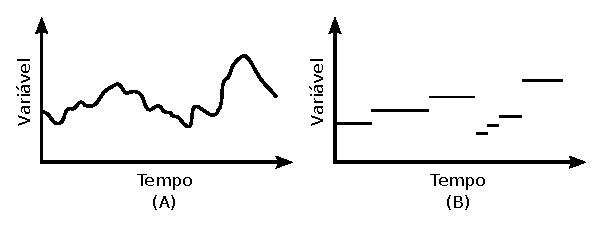
\includegraphics{img/discrete_continuous.eps}
\caption{\label{fig:disccont}Variável de estado em um modelo contínuo (A) e discreto (B). Fonte:~\cite{Banks}}
\end{figure}

\end{enumerate}

\section{Simulação Baseada em Eventos Discretos}

Segundo Law~(2000, p.~6):

\begin{directcite}
A Simulação de Eventos Discretos (\textit{Discrete-Event Simulation}) compreende
a modelagem de um sistema à medida que ele \textbf{evolui ao longo do tempo}
através de uma representação na qual as variáveis de estado são alteradas
instantaneamente em \textbf{instantes separados no tempo}.
\end{directcite}

A abordagem sugerida por Law é o padrão de projeto de simuladores ao utilizar-se
um modelo de simulação \textit{dinâmico}, \textit{estocástico} e
\textit{discreto} para representar o sistema do mundo real. Em função da
natureza dinâmica desta abordagem, é necessário acompanhar o valor atual do
tempo da simulação à medida que a simulação é executada, armazenando este valor
em uma variável. Esta variável é chamada de \textit{relógio da simulação}
\cite{Law}. Também se faz necessário um mecanismo de avanço de tempo que
gerencie o valor desta variável. Geralmente, não há relação entre o tempo de
simulação e o tempo necessário para a simulação ser executada. Por exemplo, um
experimento pode simular o funcionamento de um banco entre 9h e 17h (tempo de
simulação), mas o tempo necessário para executar a simulação poderia ser de 4
minutos.

\subsection{Mecanismo de Avanço de Tempo}

Existem duas principais abordagens para o mecanismo de avanço de tempo em um sistema de simulação de eventos discretos. São eles:

\begin{description}
\item[Avanço de tempo para o próximo evento] \hfill

Na abordagem de \textit{avanço de tempo para o próximo evento}, o
\textit{relógio da simulação} é inicializado em 0 e é determinado em que ponto
tempo ocorrerão eventos futuros - em outras palavras, é feito o agendamento de
eventos. Então, o \textit{relógio da simulação} é avançado para o tempo da
ocorrência do \textit{primeiro} destes eventos futuros. Neste ponto do tempo, o
estado do modelo é atualizado de acordo com o evento que ocorreu e novas
ocorrências de eventos futuros são agendadas. Então, o \textit{relógio da
simulação} avança para o instante exato da ocorrência do \textit{novo} primeiro
dos eventos futuros e o estado do sistema é atualizado em função da ocorrência
deste evento. Este processo repete-se até que uma condição de parada previamente
definida seja satisfeita.

Uma vez que todas e qualquer alteração no estado do sistema ocorre na ocasião de
um evento, os períodos de espera, que são o tempo entre a ocorrência de um
evento e o próximo - não são relevantes para a simulação. Afinal, o estado do
sistema não foi alterado neste ínterim - ou seja, nada de interessante ocorreu
durante aquele tempo \cite{Sim}. Deste modo, é possível reduzir o esforço
computacional necessário para executar a simulação.

\begin{figure}[htb!]
\centering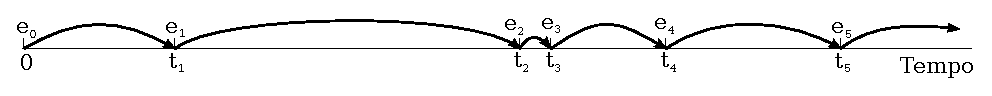
\includegraphics{img/nextevent.eps}
\caption{\label{fig:nextevent}Ilustração da evolução do \textit{relógio da simulação} utilizando a abordagem de \textit{avanço de tempo para o próximo evento}. Fonte:~\cite{Law}}
\end{figure}

Um exemplo desta dinâmica é ilustrado pela figura \ref{fig:nextevent}. O eixo do
tempo, iniciado em 0, marca os tempos agendados para os eventos $\{e_{0}, e_{1},
e_{2}, e_{3}, e_{4}, e_{5}\}$. As setas indicam os valores assumidos pelo
\textit{relógio da simulação}, ou seja, $\{t_{0}, t_{1}, t_{2}, t_{3}, t_{4},
t_{5}\}$. Observa-se que $t_{0} = e_{0}$, $t_{1} = e_{1}$ e assim sucessivamente
- ou seja, o \textit{relógio da simulação} avança diretamente para o momento
da ocorrência do próximo evento.

\item[Avanço de tempo de incremento fixo] \hfill

Na abordagem de \textit{avanço de tempo de incremento fixo}, o \textit{relógio
da simulação} é alterado sempre no mesmo incremento, independente da ocorrência
de eventos. A cada avanço é feita uma varredura para verificar se haviam eventos
agendados dentro daquele intervalo. Se um ou mais eventos estavam agendados para
ocorrer no decorrer do intervalo, considera-se que sua ocorrência se deu no
\textit{fim} do intervalo e o estado do sistema é alterado de forma
correspondente.

\begin{figure}[htb!]
\centering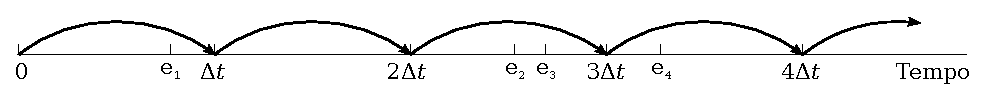
\includegraphics{img/fixed.eps}
\caption{\label{fig:fixedtime}Ilustração da evolução do \textit{relógio da simulação} utilizando a abordagem de \textit{avanço de tempo de incremento fixo}. Fonte:~\cite{Law}}
\end{figure}

A representação ilustrada pela figura \ref{fig:fixedtime} mostra a diferença
deste mecanismo para o anterior. O eixo do tempo, iniciado em 0, marca os tempos
agendados para os eventos $\{e_{1}, e_{2}, e_{3}, e_{4}\}$. As
setas indicam os valores assumidos pelo \textit{relógio da simulação}. Observa-
se que, diferentemente da abordagem anterior, o valor do \textit{relógio da
simulação} não coincide com a ocorrência de qualquer evento, e sim valores
múltiplos do incremento fixo $\Delta t$.

Algumas desvantagens desta abordagem são os erros introduzidos ao processar
eventos no fim do intervalo em que eles ocorreram e a necessidade de decidir
qual evento processar primeiro quando eventos que não ocorrem simultaneamente na
realidade são tratados como tal pelo modelo. Tais problemas poderiam ser
mitigados ao utilizar incrementos menores. Entretanto, esta medida também
aumenta o número de varreduras em intervalos para localizar eventos, o que pode
tornar sua execução muito mais custosa em termos computacionais.

Em função disto, esta abordagem é frequentemente descartada em detrimento do
\textit{avanço de tempo para o próximo evento} em modelos onde o tempo de
ocorrência de eventos pode variar bastante - que é o caso de modelos
estocásticos.

\end{description}

Sendo assim, o modelo deste estudo será uma simulação de eventos discretos com avanço de tempo para o próximo evento.

\subsection{Componentes e Organização da Simulação}

Independente do paradigma utilizado em sua implementação, um simulador de
eventos discretos possui um conjunto de componentes com responsabilidaddes bem
definidas. São eles:

\begin{description}
\item[Estado do Sistema] Coleção de variáveis necessárias para descrever o estado do sistema em um instante em particular;
\item[Relógio de Simulação] Variável contendo o valor atual do tempo de simulação;
\item[Lista de Eventos] Lista de eventos futuros, contendo, para cada evento, o
seu tipo e o instante do tempo no qual este ocorrerá;
\item[Contadores Estatísticos] Conjunto de variáveis utilizados para armazenar informações estatísticas a respeito do funcionamento do sistema;
\item[Rotina de Inicialização] Subprograma para inicializar a simulação no
instante zero do \textit{relógio da simulação};
\item[Rotina de Temporização] Subprograma responsável por determinar qual o
próximo evento a ocorrer e avançar o relógio de simulação até o instante da sua
ocorrência;
\item[Rotina de Evento] Subprograma que modifica o estado do sistema quando um determinado tipo de evento ocorre - para cada tipo de evento há uma rotina
correspondente;
\item[Rotinas Auxiliares] Conjunto de subprogramas utilizados para gerar observações aleatórias sobre distribuições de probabilidade determinadas como parte do modelo de simulação;
\item[Gerador de Relatórios] Subprograma que computa estimativas das métricas desejadas e dão origem ao relatório quando a simulação termina;
\item[Programa Principal] Subprograma que invoca as rotinas de inicialização e temporização e delega o tratamento de cada evento à sua rotina correspondente, repetindo o processo até que a condição de parada da simulação seja verificada.
\end{description}

\begin{figure}[htb!]
\centering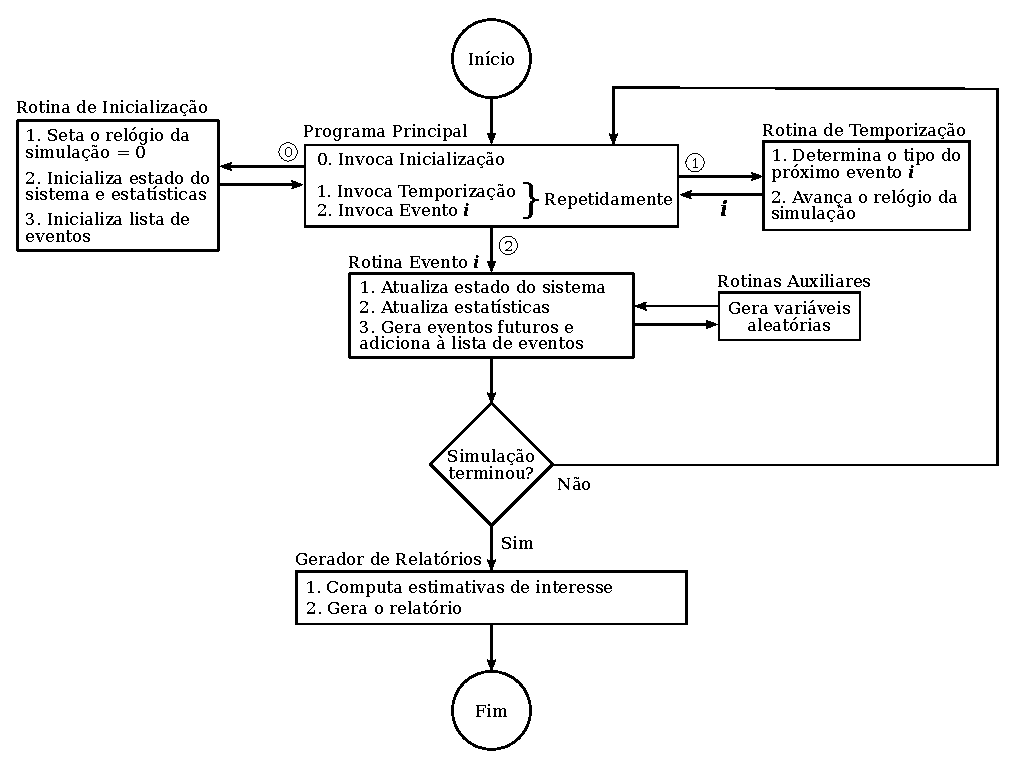
\includegraphics{img/simulation_flow.eps}
\caption{\label{fig:simflow}Fluxo básico de um simulador com avanço de tempo para o próximo evento. Fonte:~\cite{Law}}
\end{figure}

A figura \ref{fig:simflow} ilustra a organização existente entre estes
componentes, bem como o fluxo de execução da simulação. O início da simulação se
dá pela execução do \textit{Programa Principal}. Este, por sua vez, invoca a
\textit{Rotina de Inicialização}. Nesta rotina, o \textit{Relógio da Simulação}
é zerado, marcando o instante inicial. Além disso, são inicializados o
\textit{Estado Inicial} do sistema, os \textit{Contadores Estatísticos} e são
gerados os eventos iniciais, sendo adicionados à \textit{Lista de Eventos}.

Após o controle retornar para o \textit{Programa Principal}, o mesmo invoca a
\textit{Rotina de Temporização}. Esta rotina tem a responsabilidade de avaliar a
\textit{Lista de Eventos} e determinar qual é o primeiro evento a ser executado.
Ao determinar qual é o evento, a rotina avança o \textit{Relógio da Simulação}
para o instante de sua ocorrência e devolve informações a respeito deste evento
para o \textit{Programa Principal}. De volta ao \textit{Programa Principal}, o
mesmo avalia o evento retornado pela \textit{Rotina de Temporização} e invoca
sua \textit{Rotina de Evento} correspondente.

Para cada tipo de evento existe uma \textit{Rotina de Evento} correspondente.
Todas elas, obrigatoriamente, devem executar as seguintes tarefas: (1) atualizar
o \textit{Estado do Sistema} em função do evento ocorrido; (2) atualizar os
\textit{Contadores Estatísticos} em função do evento ocorrido; e (3) gerar
novos eventos futuros e adicioná-los à \textit{Lista de Eventos}. Para esta
última tarefa, as \textit{Rotinas Auxiliares} são utilizadas para diversas
tarefas - dentre elas, a geração de variáveis aleatórias para dar suporte à
geração de eventos estocásticos.

Após a execução da \textit{Rotina de Evento}, é feita a verificação de uma
condição de parada da simulação. Caso seja determinado que o fim da simulação
deve ocorrer, o controle passa para o \textit{Gerador de Relatórios}, cuja
responsabilidade é computar as estimativas de interesse, baseando-se nos
\textit{Contadores Estatísticos} e produzir um relatório com estes dados. Em
caso contrário, o \textit{Programa Principal} é invocado novamente e o ciclo se
repete. É importante salientar que a \textit{Rotina de Inicialização} somente é
invocada na primeira execução do \textit{Program Principal}, sendo ignorada nas
iterações posteriores.

%\begin{algorithm}[htb]
%\begin{center}
%\begin{algorithmic}[1]
%\Function{Initialize}{$clock, state, statistics$}
%  \State $clock \gets 0.0$
%  \State Initialize $state$
%  \State Initialize $statistics$
%\EndFunction
%\Statex
%\Function{Timing}{$clock, state, statistics$}
%  \State $clock \gets 0.0$
%  \State Initialize $state$
%  \State Initialize $statistics$
%\EndFunction
%\Statex
%\Function{Main}{}
%  \State $clock \gets null$
%  \State $state \gets null$
%  \State $statistics \gets null$
%  \State $eventList \gets \text(new queue<Event>)$
%  \State \Call{InitializationRoutine}{clock, state, statistics}
%  \While{$\Call{ShouldSimulationRun}{clock, state}$}
%    \State $nextEvent \gets \Call{GetNextEvent}{}$
%    \If{<text>}
%    <body>
%    \ElsIf{<text>}
%    <body>
%    \Else
%    <body>
%    \EndIf
%  \EndWhile
%\EndFunction
%\Procedure{Euclid}{$a,b$}\Comment{The g.c.d. of a and b}
%\State $r\gets a\bmod b$
%\While{$r\not=0$}\Comment{We have the answer if r is 0}
%\State $a\gets b$
%\State $b\gets r$
%\State $r\gets a\bmod b$
%\EndWhile\label{euclidendwhile}
%\State \textbf{return} $b$\Comment{The gcd is b}
%\EndProcedure
%\end{algorithmic}
%\end{center}
%\caption[An algorithm with an optional, shorter caption]%
%    {\label{alg:alg1}This is an algorithm with a very long
%    caption. However, we replaced it with a shorter version
%    in the Outline for legibility reasons}%
%\end{algorithm}